\documentclass{article}
\usepackage{graphicx} % Required for inserting images
\usepackage{amsmath}
\usepackage{dirtytalk}
\usepackage{float}
\usepackage[italian]{babel}
\usepackage{hyperref}

\renewcommand{\figurename}{Figura}

\title{Prova Finale di Reti Logiche}
\author{Federico Grandi [10802488]}
\date{Settembre 2024}

\begin{document}

\maketitle

\tableofcontents 

\section{Introduzione}

La consegna richiede di progettare un componente hardware che vada ad eseguire delle operazioni sulla memoria ad esso collegata, basandosi sui segnali che riceve in entrata e sul contenuto della memoria stessa.

\subsection{Struttura del componente}
Il componente deve possedere le porte per i seguenti segnali:
\begin{itemize}
    \item 3 ingressi primari: \texttt{START} (1 bit), \texttt{ADD} (16 bit), \texttt{K} (10 bit).
    \item 1 uscita primaria: \texttt{DONE} (1 b{it}).
    \item 1 segnale di \texttt{CLOCK}, unico per tutto il sistema, con periodo di almeno 20 ns.
    \item 1 segnale di \texttt{RESET}, unico per tutto il sistema.
    \item I segnali per comunicare con la memoria: \texttt{O\_MEM\_ADDR} (16 bit), \\
    \texttt{I\_MEM\_DATA} (8 bit), \texttt{O\_MEM\_DATA} (8 bit), \texttt{O\_MEM\_WE} (1 bit), \\ 
    \texttt{O\_MEM\_EN}(1 bit).
\end{itemize}


\subsection{Comportamento del componente}
Il componente deve manipolare i dati contenuti in memoria negli indirizzi da $\texttt{ADD}$ a $\texttt{ADD}+\texttt{K}*2-1$ (inclusi), secondo i seguenti criteri:

\begin{enumerate}
    \item Tutti i dati in memoria nelle posizioni $\texttt{ADD} + k*2, k \in [0, \texttt{K})$ sono considerati valori di una sequenza, ad eccezione degli 0, che vengono trattati come non-valori.
    \item Per ogni valore salvato in memoria in posizione $\texttt{ADD}+i$, se il dato in posizione $\texttt{ADD}+i+1$ non è 0, allora esso va sostituito con un valore di \say{credibilità} 31.
    \item Per ogni valore salvato in memoria in posizione $\texttt{ADD}+i$, se il dato in posizione $\texttt{ADD}+i+1$ è 0, allora esso va sostituito con un valore di "credibilità" pari al valore di credibilità precedente diminuito di 1, se esiste ed è maggiore di 0, altrimenti 0.
    \item Ogni non valore nella sequenza va sostituito con il valore precedente, se esso esiste.
\end{enumerate}

L'uscita \texttt{DONE} dev'essere impostata ad 1 solamente quando il componente ha terminato tutte le elaborazioni e scritture in memoria.

\texttt{RESET} è l'unico segnale asincrono, e quando viene portato a 1 il componente dev'essere reimpostato allo stato originale. Tutti gli altri segnali sono da considerarsi sincroni, da interpretare sul fronte di salita di \texttt{CLOCK}. \\

L'elaborazione deve iniziare quando \texttt{START} viene portato a 1, momento dopo il quale \texttt{ADD} e \texttt{K} possono essere considerati costanti. \texttt{START} rimarrà a 1 finché il componente non porrà \texttt{DONE} a 1.

Riassumendo, sono stati presi in considerazione i seguenti elementi:
\label{par:casi-notevoli}
\begin{itemize}
    \item La credibilità deve rimanere a 0 finché non si incontra il primo valore.
    \item È necessario andare a scrivere in memoria solamente se il dato presente non è 0.
    \item La credibilità ha 0 come valore minimo.
    \item Il componente deve poter processare più sequenze tramite un corretto utilizzo del segnale \texttt{START}.
\end{itemize}

\paragraph{Esempio di sequenza}
Di seguito (figura \ref{fig:example-sequence}) viene riportata la sequenza di dati nella porzione di memoria interessata prima e dopo l'elaborazione da parte del componente. I dati sono scritti in valori decimali; per brevità, ho riportato come [...] una serie di \say{0 0} nella sequenza di dati in ingresso.

Nella figura seguente viene evidenziato, tramite colorazione:
\begin{itemize}
    \item In verde, il modo in cui i valori vengono riportati.
    \item In blu, i punti dove il valore di credibilità viene diminuito.
    \item In rosso, un punto dove il valore di credibilità non viene mostrato anche se viene diminuito, perché il dato in entrata non è 0.
    \item In giallo, i punti in cui il valore di credibilità viene resettato a 31.
\end{itemize}

% codice che ha generato la tabella in immagine
\iffalse
\begin{tabular}{rcc}
    Indirizzo & Prima & Dopo \\
    ADD & 0 & 0 \\
    ADD + 1 & 0 & 0 \\
    ADD + 2 & 1 & 1 \\
    ADD + 3 & 0 & 31 \\
    ADD + 4 & 0 & 1 \\
    ADD + 5 & 0 & 30 \\
    ADD + 6 & 2 & 2 \\
    ADD + 7 & 0 & 31 \\
    ADD + 8 & 0 & 2 \\
    ADD + 9 & 5 & 5 \\
    ADD + 10 & 0 & 2 \\
    ADD + 11 & 0 & 29 \\
    \vdots & \vdots & \vdots \\
    ADD + 66 & 0 & 2  \\
    ADD + 67 & 0 & 1 \\
    ADD + 68 & 0 & 2 \\
    ADD + 69 & 0 & 0 \\
    ADD + 70 & 0 & 2 \\
    ADD + 71 & 0 & 0 \\
    ADD + 72 & 7 & 7 \\
    ADD + 73 & 0 & 31
\end{tabular}
\fi

\begin{figure}[H]
    \centering
    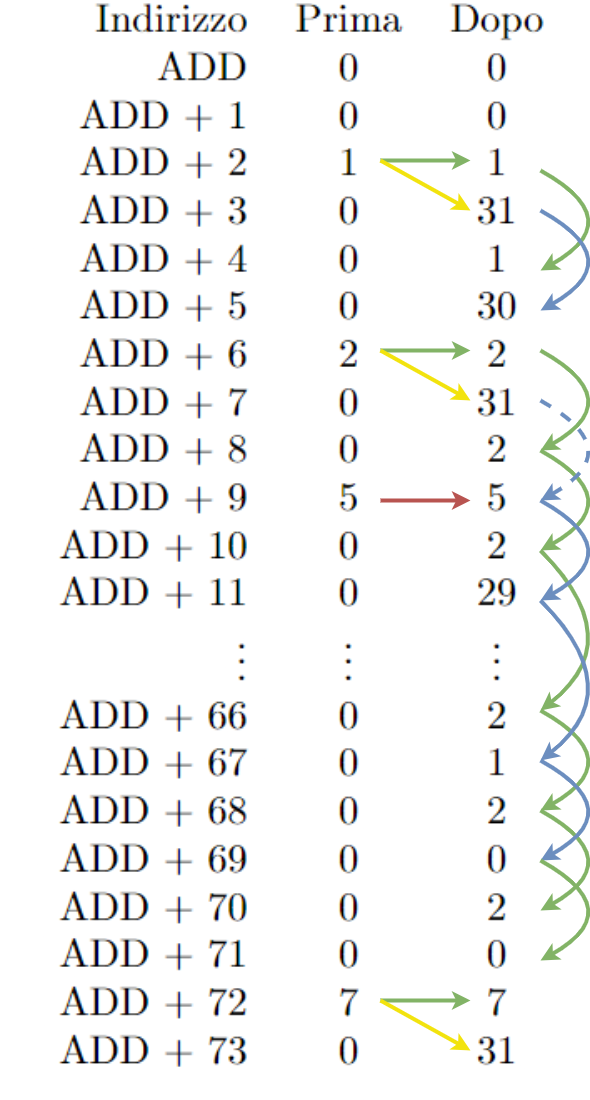
\includegraphics[width=0.5\linewidth]{Example sequence.drawio.png}
    \caption{Sequenza di esempio}
    \label{fig:example-sequence}
\end{figure}


\section{Architettura}

\subsection{Moduli}

Per quanto riguarda l'architettura si è preferito optare per una soluzione mono-componente multi-processo: non essendo le operazioni da eseguire particolarmente articolate, si è scelto di mantenere una minore complessità e quindi di evitare di aggiungere ulteriori moduli. \\
Lo schema dei moduli che ne risulta è riportato di seguito nella figura \ref{fig:components}.
Nello schema è anche riportato il modulo di memoria, con cui vengono mostrati i collegamenti, che è però descritto nei testbench e non fa quindi parte del sorgente VHDL.

\begin{figure}[H]
    \centering
    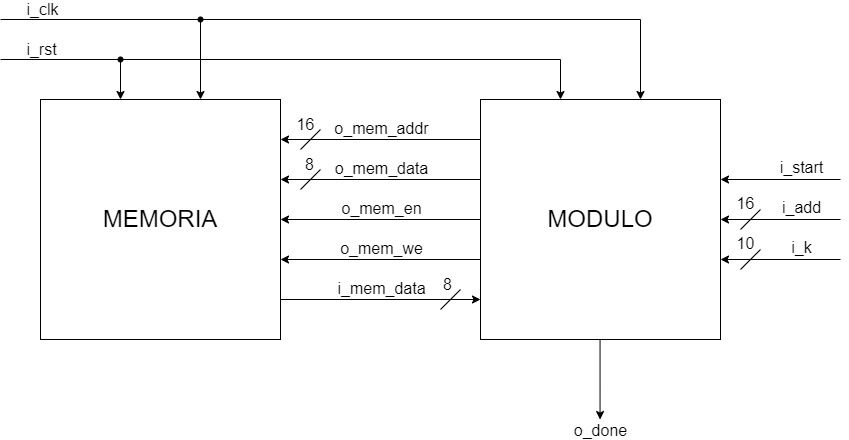
\includegraphics[width=\linewidth]{Component diagram.drawio.png}
    \caption{Moduli}
    \label{fig:components}
\end{figure}

\subsection{Processi}

All'interno dell'architettura del componente vengono descritti 6 processi in tutto:
\begin{itemize}
    \item 4 per gestire i registri:
    \begin{enumerate}
        \item Stato della Macchina a Stati Finiti.
        \item Contatore per tener traccia di quanti elementi della sequenza sono stati processati.
        \item Valore di credibilità C.
        \item Ultimo valore letto.
    \end{enumerate}

    \item 2 per rappresentare le funzioni della MSF:
    \begin{enumerate}
        \setcounter{enumi}{4}
        \item Funzione di transizione $\delta$, che si occupa di determinare lo stato successivo in base allo stato corrente, al numero di valori processati, e alle entrate del componente
        \item Funzione di uscita $\lambda$, che si occupa di determinare i valori da assegnare alle uscite e ai registri, basandosi sui valori dei registri e delle entrate del componente
    \end{enumerate}
\end{itemize}

Sono stati inoltre dichiarati 8 segnali interni, 2 per ciascun registro. \\

I 6 stati della MSF sono rappresentati nel diagramma in figura \ref{fig:msf}. Si possono notare gli autoanelli sugli stati \texttt{INIT} e \texttt{DONE}, che bloccano la macchina in base al valore di \texttt{i\_start}, e la biforcazione del flusso in \texttt{WRITE\_CRED}, in base al fatto che tutti i valori della sequenza siano già stati letti o meno.

\begin{figure}[H]
    \centering
    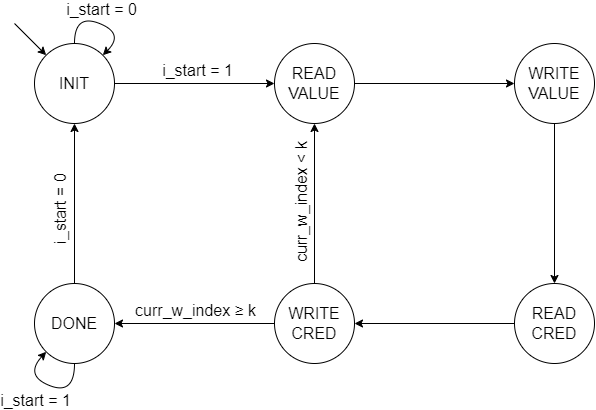
\includegraphics[width=0.75\linewidth]{FSM.drawio.png}
    \caption{Diagramma degli stati della MSF}
    \label{fig:msf}
\end{figure}

Negli stati vengono effettuate le seguenti operazioni:

\begin{itemize}
    \item \texttt{INIT}: reimposta i valori dei registri \texttt{cred}, \texttt{w\_index}, e \texttt{last\_w} a 0.
    \item \texttt{READ\_VALUE}: imposta l'indirizzo del valore della sequenza da leggere (partendo da \texttt{i\_add}) e abilita la lettura della memoria.
    \item \texttt{WRITE\_VALUE}: se il dato letto non è 0, lo salva in \texttt{last\_w} e imposta \texttt{cred} a 31; in caso contrario, diminuisce \texttt{cred} e scrive in memoria l'ultimo dato letto.
    \item \texttt{READ\_CRED}: imposta l'indirizzo successivo a quello del dato appena letto, predisponendone la lettura.
    \item \texttt{WRITE\_CRED}: incrementa \texttt{w\_index} e, se il dato presente in memoria è 0, allora lo sovrascrive con il valore di credibilità.
    \item \texttt{DONE}: imposta \texttt{o\_done} a 1.
\end{itemize}

Gli stati \texttt{WRITE\_VALUE} e \texttt{WRITE\_CRED} vengono sempre percorsi, anche quando non è necessario scrivere in memoria, perché devono svolgere anche dei compiti aggiuntivi (come aggiornare i registri di \texttt{cred} e \texttt{w\_index}).


\section{Dati sperimentali}

\subsection{Sintesi}

Per ottenere i dati riguardanti la sintesi del componente, è possibile fare riferimento a due report, uno relativo all'utilizzo delle risorse (\texttt{report\_utilization}) e uno relativo alle tempistiche (\texttt{report\_timing}).

Da quello sull'utilizzo delle risorse è possibile notare (vedi tabella \say{1. Slice Logic} riportata sotto) che non sono presenti latch nella sintesi del design. Da ciò è possibile trarre che, all'interno di ciascun processo, i segnali sono assegnati in modo completo per tutti i percorsi logici, evitando comportamenti non deterministici.

%+-------------------------+------+-------+------------+-----------+-------+
%|        Site Type        | Used | Fixed | Prohibited | Available | Util% |
%+-------------------------+------+-------+------------+-----------+-------+
%| Slice LUTs*             |   78 |     0 |          0 |    134600 |  0.06 |
%|   LUT as Logic          |   78 |     0 |          0 |    134600 |  0.06 |
%|   LUT as Memory         |    0 |     0 |          0 |     46200 |  0.00 |
%| Slice Registers         |   26 |     0 |          0 |    269200 | <0.01 |
%|   Register as Flip Flop |   26 |     0 |          0 |    269200 | <0.01 |
%|   Register as Latch     |    0 |     0 |          0 |    269200 |  0.00 |
%| F7 Muxes                |    0 |     0 |          0 |     67300 |  0.00 |
%| F8 Muxes                |    0 |     0 |          0 |     33650 |  0.00 |
%+-------------------------+------+-------+------------+-----------+-------+
\begin{center}
\begin{tabular}{|l|r|r|r|r|r|}
    \hline
    \multicolumn{1}{|c|}{\textbf{Site type}} & \multicolumn{1}{|c|}{\textbf{Used}} & \multicolumn{1}{|c|}{\textbf{Fixed}} & \multicolumn{1}{|c|}{\textbf{Prohibited}} & \multicolumn{1}{|c|}{\textbf{Available}} & \multicolumn{1}{|c|}{\textbf{Util}\%} \\
    \hline
    Slice LUTs* & 78 & 0 & 0 & 134600 & 0.06 \\
    \hspace{5pt} LUT as Logic & 78 & 0 & 0 & 134600 & 0.06 \\
    \hspace{5pt} LUT as Memory & 0 & 0 & 0 & 46200 & 0.00 \\
    Slice Registers & 26 & 0 & 0 & 269200 & $<$0.01 \\
    \hspace{5pt} Register as Flip Flop & 26 & 0 & 0 & 269200 & $<$0.01 \\
    \hspace{5pt} Register as Latch & 0 & 0 & 0 & 269200 & 0.00 \\
    F7 Muxes & 0 & 0 & 0 & 67300 & 0.00 \\
    F8 Muxes & 0 & 0 & 0 & 33650 & 0.00 \\
    \hline
\end{tabular}
\end{center}

\vspace{5pt}
Di seguito vengono riportati altri dati degni di nota, estratti dalle altre tabelle non riportate per brevità:

\begin{enumerate}
    \item Non è stata utilizzata la BRAM disponibile.
    \item Non è stato utilizzato nessun DSP.
    \item Risulta utilizzato un solo segnale di clock.
\end{enumerate}

Dall'analisi delle tempistiche si può notare che il componente opera con uno slack di 16.756ns e che il data path delay, ovvero il massimo tempo di propagazione lungo i percorsi del design, è di 3.093ns. Il requisito di 20ns è quindi ampiamente soddisfatto.

\subsection{Simulazione}

Per simulare l'operato del componente è stato fatto uso di diversi testbench, tutti strutturati in modo simile, che si occupano di simulare le operazioni di memoria e di controllare il componente collegandosi ad input e output dello stesso. Per ciascuna elaborazione che si vuole testare, si occupano di caricare in memoria i vari \say{scenari} e, ad elaborazione conclusa, di verificare che in memoria siano presenti i valori attesi, specificati a priori nel codice del testbench.

Di seguito sono riportati i risultati di alcune simulazioni significative al fine di mostrare il funzionamento del componente.

\subsubsection{Sequenza di esempio}

\begin{figure}[b]
    \centering
    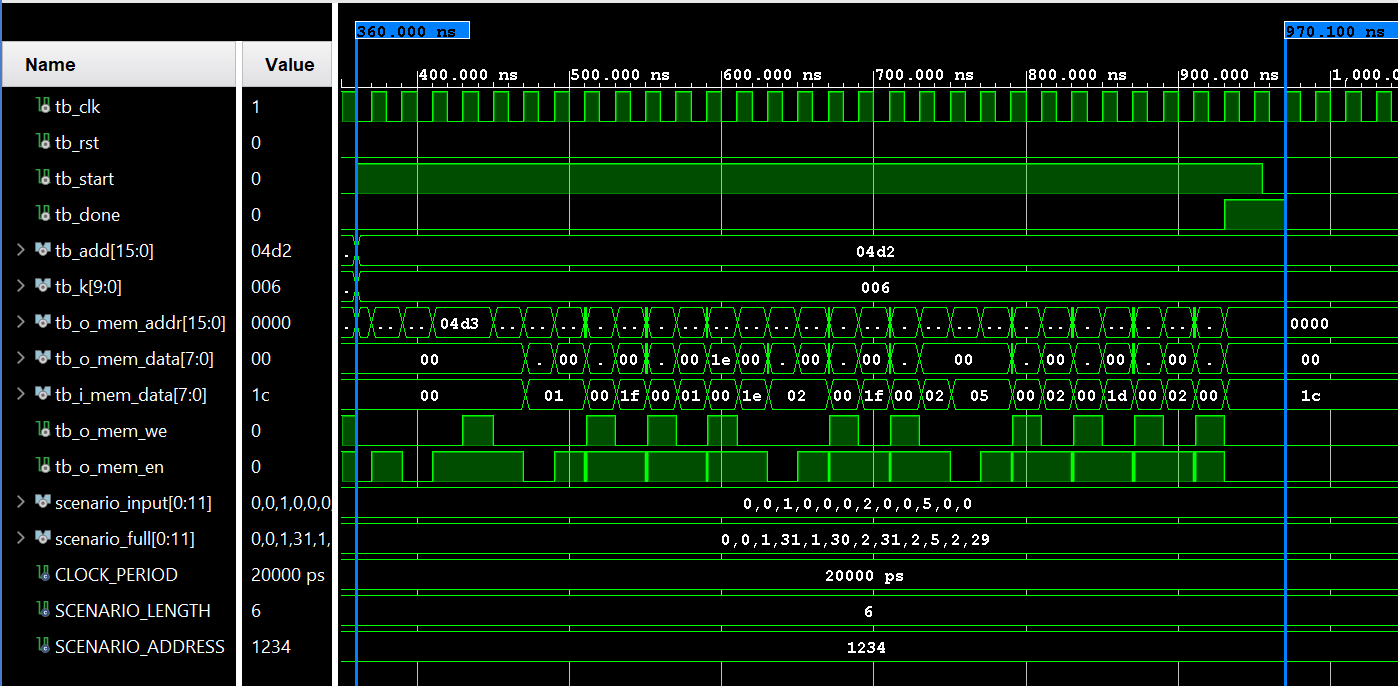
\includegraphics[width=1\linewidth]{tb/custom_tb.png}
    \caption{Oscilloscopio - sequenza di esempio}
    \label{fig:suctom-tb}
\end{figure}

In questa simulazione (figura \ref{fig:suctom-tb}) è possibile vedere chiaramente i 5 momenti in cui l'accesso alla memoria (\texttt{tb\_o\_mem\_en}) è disabilitato:
\begin{itemize}
    \item Nel primo caso, la MSF è nello stato \texttt{WRITE\_VALUE} e il dato letto è 0, ma non è ancora stato letto nessun valore
    \item Nel secondo e nel terzo caso, la MSF è in \texttt{WRITE\_VALUE}, ma è stato letto un nuovo valore
    \item Nel quarto caso, la MSF è in \texttt{WRITE\_CRED}, ma il valore letto è diverso da 0
    \item Nell'ultimo caso, la MSF è in \texttt{DONE}, e quindi non sono necessarie più operazioni sulla memoria
\end{itemize}

È anche possibile notare delle linee di colore più intenso all'interno del segnale tb\_o\_mem\_en, dovute a rapidi cambiamenti nel valore, causati dai tempi di propagazione dei segnali. Questi cambiamenti avvengono comunque non a cavallo del fronte di salita e quindi non rappresentano un problema per il funzionamento del componente.

\subsubsection{Sequenza di lunghezza 0}
Vedi figura \ref{fig:empty-tb}.
\begin{figure}[b]
    \centering
    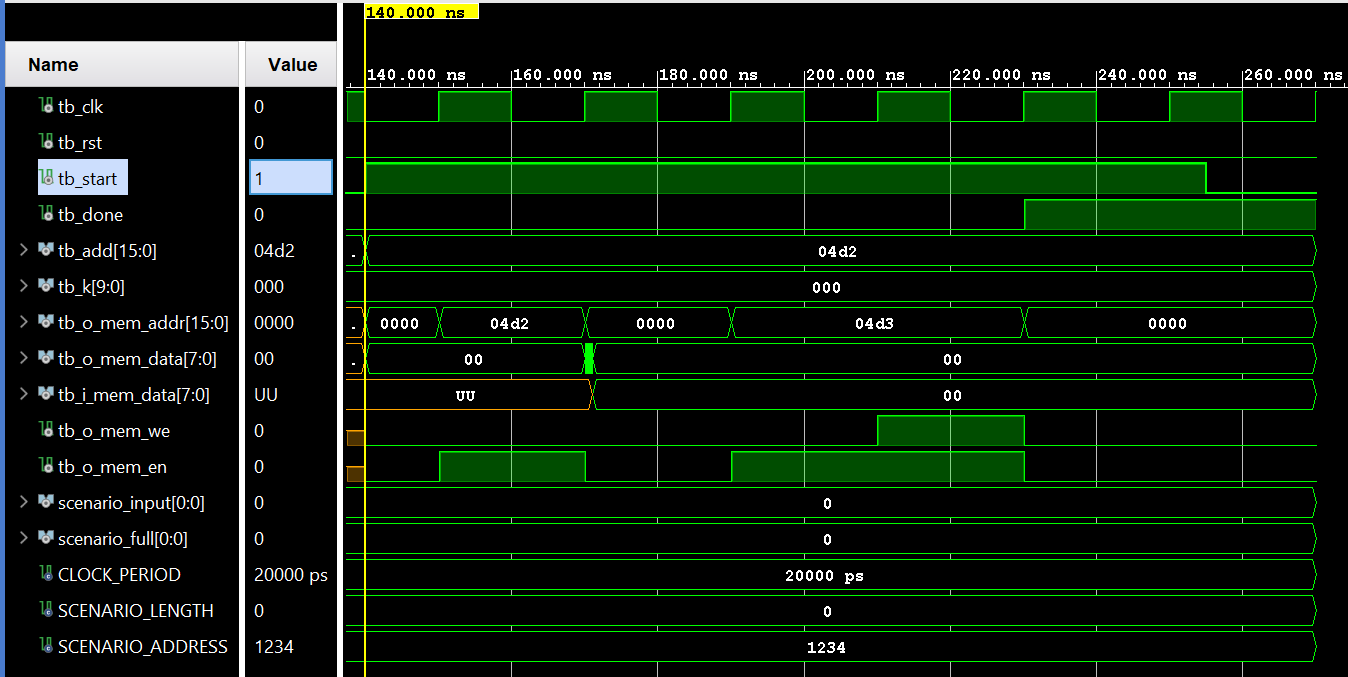
\includegraphics[width=1\linewidth]{tb/empty_tb.png}
    \caption{Oscilloscopio - sequenza vuota}
    \label{fig:empty-tb}
\end{figure}

\subsubsection{Elaborazioni consecutive}
Vedi figura \ref{fig:multi-start-tb}.
\begin{figure}
    \centering
    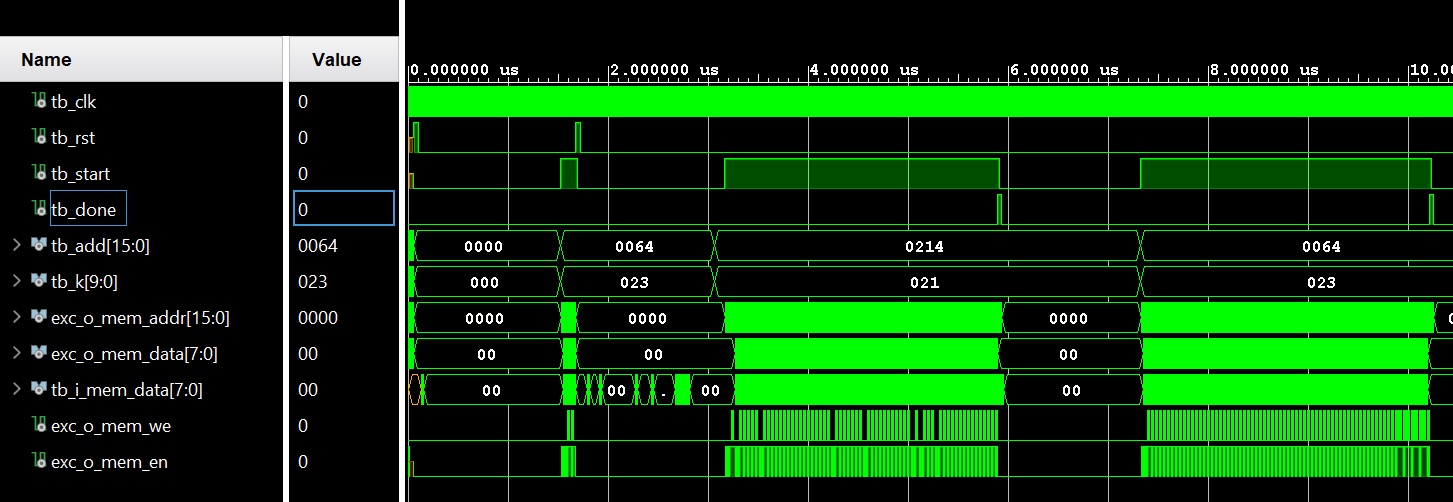
\includegraphics[width=1\linewidth]{tb/multi_start_tb.png}
    \caption{Oscilloscopio - elaborazioni consecutive}
    \label{fig:multi-start-tb}
\end{figure}

\subsubsection{Gestione del segnale di reset}
Vedi figure \ref{fig:reset-during-read-tb} e \ref{fig:start-during_reset_tb}.
\begin{figure}
    \centering
    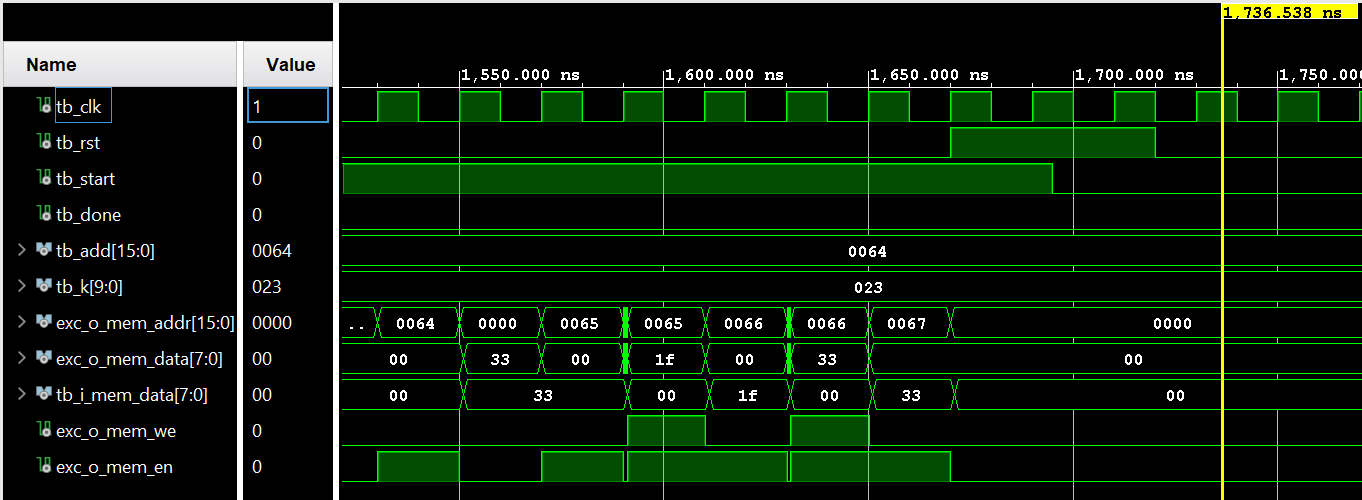
\includegraphics[width=1\linewidth]{tb/reset_during_read_tb.png}
    \caption{Oscilloscopio - reset durante lettura}
    \label{fig:reset-during-read-tb}
\end{figure}
\begin{figure}
    \centering
    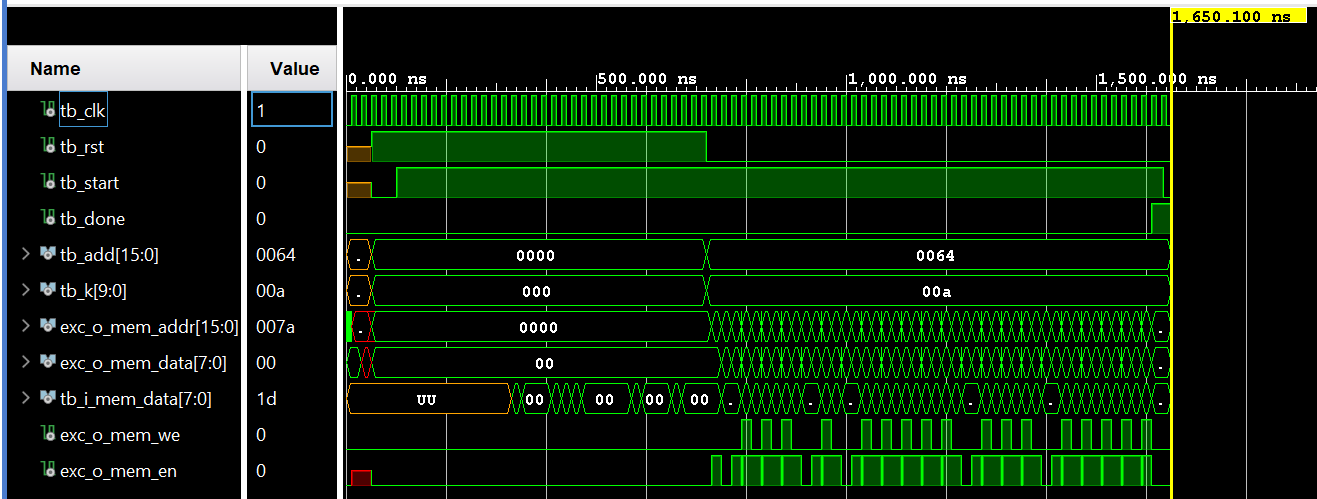
\includegraphics[width=1\linewidth]{tb/start_during_reset_tb.png}
    \caption{Oscilloscopio - start durante reset}
    \label{fig:start-during_reset_tb}
\end{figure}

\section{Conclusioni}

I risultati sperimentali riguardanti la sintesi sono soddisfacenti, perché evidenziano un'assenza di latch non necessari e un tempo di propagazione massimo molto al di sotto del limite richiesto. \\

Sono soddisfacenti anche gli esiti delle simulazioni, che dimostrano che il componente è in grado di gestire diversi scenari correttamente. In particolare, il componente:

\begin{itemize}
    \item produce una sequenza finale rispettando la specifica, tenendo in considerazione i casi notevoli delineati \hyperref[par:casi-notevoli]{nell'introduzione}.
    \item è in grado di gestire più elaborazioni consecutive.
    \item gestisce correttamente i segnali di reset indipendentemente dallo stato in cui si trova internamente.
    \item non accede a zone di memoria al di fuori del range della sequenza né in lettura né in scrittura.
\end{itemize}

\end{document}
